\documentclass{beamer}

%\usetheme{ENSLyon}

\usetheme{AnnArbor}

\title[UFSC 2020]{\Large Primeiros passos ao utilizar o Julia no Windows}
\author[G. Philippi]{{\bf Guilherme Philippi}}
\institute[]{Acadêmico de Engenharia de Controle e Automação\\ Campus Blumenau \\  Universidade Federal de Santa Catarina \\ Orientado por Felipe Delfini Caetano Fidalgo \vspace{0.3cm}}
\date[03 Março, 2020]{\scriptsize UFSC 2020 \\ Métodos Numéricos\\ Blumenau - Santa Catarina - Brasil}
\setbeamersize{text margin left=5mm}
\setbeamersize{text margin right=5mm}

\setbeamertemplate{navigation symbols}{}
%\usecolortheme{ENSLyon_greener}
\usecolortheme{wolverine}

%PACKAGES -------------------------
\usepackage{etex}
\usepackage[utf8]{inputenc}
\usepackage[english]{babel}
\usepackage{enumerate}
\usepackage{amsmath}
\usepackage{amssymb}
\usepackage{amsthm}
\usepackage{amscd}
\usepackage{amsfonts}
\usepackage{multicol}
\usepackage{multirow}
\usepackage{array}
\usepackage{color}
\usepackage{graphicx}
\usepackage{tikz}
\usepackage{tikz-qtree}
\usepackage{wrapfig}
\usepackage{3dplot}
\usepackage{pgf}
\usepackage{tkz-euclide}
\usepackage{algorithmic}
\usepackage{algorithm}
\usepackage{xparse}
\usepackage{subfigure}

%LIBRARIES-TIKZ ------------------------------------------

\usetikzlibrary{shadows,trees}
\usetikzlibrary{decorations.pathmorphing}
\usetikzlibrary{decorations.markings}
\usetikzlibrary{positioning}
\usetikzlibrary{chains,matrix,scopes}
\usetikzlibrary{arrows}

%DEFINITIONS ----------------------------------------------------

\def\centerarc[#1](#2)(#3:#4:#5)% Syntax: [draw options] (center) (initial angle:final angle:radius)
{ \draw[#1] ($(#2)+({#5*cos(#3)},{#5*sin(#3)})$) arc(#3:#4:#5); }
\def\xx{\mathbf{x}}
\def\ii{\mathbf{i}}
\def\jj{\mathbf{j}}
\def\kk{\mathbf{k}}
\def\tt{\mathbf{t}}
\def\ee{\mathbf{e}}
\def\qq{\mathbf{q}}
\def\pp{\mathbf{p}}
\def\vv{\mathbf{v}}
\def\rr{\mathbf{r}}
\def\vzero{\mathbf{0}}
\def\qset{\mathbb{H}}
\def\xx{\mathbf{x}}

%NEW THEOREMS ------------------------------------------

\newtheorem{definicao}{Definition}
\newtheorem{prop}{Proposição}
\newtheorem{teo}{Teorema}
\newtheorem{cor}{Corolário}


\begin{document}
	
	%FACE
	\begin{frame}
	
		\titlepage
		
		\vspace{-0.7cm}
		\begin{flushleft}
			
\includegraphics[scale=0.08]{brasaoazul_ufsc}
		\end{flushleft}
		
	\end{frame}
	
	%Indice
	\begin{frame}
		\tableofcontents 
	\end{frame}
	
	\section{Preliminares}
	
	%SLIDE 1
	\begin{frame}
		\frametitle{\normalsize Preliminares} 
		\begin{center} 
			\large Para que queremos descobrir localizações?
		\end{center}
		
		\begin{figure}
			\subfigure{
\includegraphics[width=4.9cm]{brasaoazul_ufsc}}
			\hspace{0.3cm}
			\subfigure{
\includegraphics[width=4.7cm]{brasaoazul_ufsc}}
			\\
			\subfigure{
\includegraphics[width=5.5cm]{brasaoazul_ufsc}}
			\subfigure{
\includegraphics[width=5.5cm]{brasaoazul_ufsc}}
		\end{figure}
	\end{frame}
	
	
	%Slide End
	\begin{frame}
		\centering
		\begin{minipage}{0.3\linewidth}
			\begin{flushleft}
				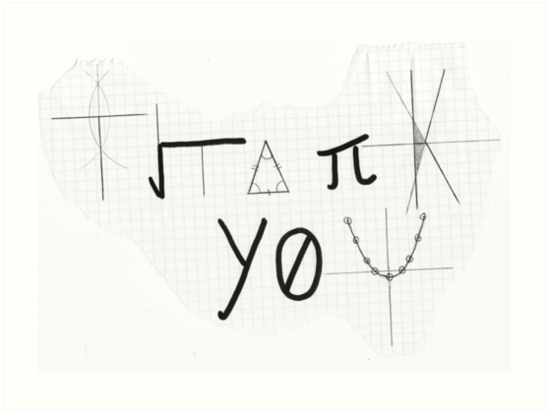
\includegraphics[scale=0.35]{thank}
			\end{flushleft}
		\end{minipage}
		\hspace{2.5cm}
		\begin{minipage}{0.4\linewidth} \centering 
			{\color{blue} \underline{guilherme.philippi@hotmail.com}} \vspace{0.2cm}  \\ UFSC - Blumenau
		\end{minipage}
	\end{frame}

\end{document}
